\documentclass[12pt,a4paper]{article}
\usepackage[utf8]{inputenc}
\usepackage[T1]{fontenc}
\usepackage{babel}
\usepackage{amsmath}
\usepackage{amsfonts}
\usepackage{fancyhdr}
\usepackage{amssymb}
\usepackage{color}
\usepackage{mdframed}
\usepackage{multirow} 
\usepackage{multicol} 
\usepackage{tikz}
\usepackage{graphicx}
\usepackage[absolute]{textpos} 
\usepackage{colortbl}
\usepackage{array}
\usepackage{geometry}
\usepackage{hyperref}
\usepackage{tabularx}
\usepackage{minted}
\usepackage[most]{tcolorbox}
\usepackage{hyperref}
\usepackage{enumitem}
\usepackage{booktabs}
\usepackage{xcolor}
\usepackage{subfig}


\definecolor{BleuFonce}{RGB}{0,74,117}
\definecolor{lightgreen}{rgb}{0.56, 0.93, 0.56}
\definecolor{moonstoneblue}{rgb}{0.45, 0.66, 0.76}
\definecolor{vtmaroon}{RGB}{99,0,49}


\pagestyle{fancy}
\renewcommand\headrulewidth{1pt}
\usepackage{float}

%\fancyfoot[L]{Virginia Tech \& Open University }
\fancyhead[R]{}
%\fancyhead[L]{Prénom Nom}



\newcommand{\begincodebox}[1]{
\vspace{1ex}
\begin{tcolorbox}[
    enhanced,
    attach boxed title to top left={xshift=6mm,yshift=-3mm},
    colback=moonstoneblue!20,
    colframe=moonstoneblue,
    colbacktitle=moonstoneblue,
    title=#1,
    fonttitle=\bfseries\color{black},
    boxed title style={size=small,colframe=moonstoneblue,sharp corners},
    sharp corners,
]
}

\newcommand{\codeboxend}{\end{tcolorbox}\noindent}
\newcommand{\foxdec}{\textsf{FoxDec}}
\newcommand{\beginpar}[1]{\noindent\textsc{\textbf{#1.}}}



\newcounter{example}
\NewDocumentEnvironment{example}{ O{} }
{
\colorlet{colexam}{vtmaroon} % Global example color
\newtcolorbox[use counter=example]{examplebox}{%
    % Example Frame Start
    empty,% Empty previously set parameters
    title={Example: #1},% use \thetcbcounter to access the example counter text
    % Attaching a box requires an overlay
    attach boxed title to top left,
       % Ensures proper line breaking in longer titles
       minipage boxed title,
    % (boxed title style requires an overlay)
    boxed title style={empty,size=minimal,toprule=0pt,top=4pt,left=3mm,overlay={}},
    coltitle=colexam,fonttitle=\bfseries,
    before=\par\medskip\noindent,parbox=false,boxsep=0pt,left=3mm,right=0mm,top=2pt,breakable,pad at break=0mm,
       before upper=\csname @totalleftmargin\endcsname0pt, % Use instead of parbox=true. This ensures parskip is inherited by box.
    % Handles box when it exists on one page only
    overlay unbroken={\draw[colexam,line width=.5pt] ([xshift=-0pt]title.north west) -- ([xshift=-0pt]frame.south west); },
    % Handles multipage box: first page
    overlay first={\draw[colexam,line width=.5pt] ([xshift=-0pt]title.north west) -- ([xshift=-0pt]frame.south west); },
    % Handles multipage box: middle page
    overlay middle={\draw[colexam,line width=.5pt] ([xshift=-0pt]frame.north west) -- ([xshift=-0pt]frame.south west); },
    % Handles multipage box: last page
    overlay last={\draw[colexam,line width=.5pt] ([xshift=-0pt]frame.north west) -- ([xshift=-0pt]frame.south west); },%
    }
\begin{examplebox}}
{\end{examplebox}\endlist}



\begin{document}

\begin{titlepage}


%\thispagestyle{empty}

\newgeometry{left=6cm,bottom=2cm, top=1cm, right=1cm}

\tikz[remember picture,overlay] \node[opacity=1,inner sep=0pt] at (2.2mm,-165mm){
\includegraphics{SideBar.png}}; 

\fontfamily{fvs}\fontseries{m}\selectfont

\color{white}

%%Texte vertical à gauche
\begin{picture}(0,0)
\put(-110,-743){\rotatebox{90}{\Huge{FoxDec User Manual}}}
\end{picture}
 
%**************************************************************
%********************  LOGO  DE  POLYTECH  ********************
%****** CHANGER L'IMAGE POUR UN AUTRE POLYTECH QUE SACLAY *****
%* VOIR LES LOGOS DISPONIBLES, ET REMPLACER LE NOM CI-DESSOUS *
%**************************************************************

\vspace{-10mm} 
\flushright 
\begin{tabular}{cc}
\multicolumn{1}{|m{5cm}|}{\makebox(100,100){
\includegraphics[width=140px]{VT.jpeg}}} &
\multicolumn{1}{|m{5cm}|}{\makebox(140,100){
\includegraphics[width=140px]{OU.jpg}}} 
\end{tabular}




%*****************************************************
%******************** TITRE **************************
%*****************************************************
\flushright
\vspace{10mm} % à régler éventuellement
\color{BleuFonce}
\fontfamily{cmss}\fontseries{m}\fontsize{22}{26}\selectfont
  \textbf{FoxDec}

\normalsize
\color{black}
%*****************************************************

%\fontfamily{fvs}\fontseries{m}\fontsize{8}{12}\selectfont

\vspace{1.5cm}
\normalsize

\textbf{Decompilation based on Formal Methods}

\vspace{15mm}

\begin{tabular}{rr}
prof. Binoy Ravindran & PI\\
dr. Freek Verbeek & co-PI\\[1ex]
Joshua Bockenek& PhD\\
Daniel Spaniol& PhD\\
\end{tabular}
\\[1ex]
\href{mailto:freek@vt.edu}{freek@vt.edu}

\vspace{15mm}

\textbf{Supported by the DARPA project FALCON: \\ Formal Analysis of Legacy COde domaiNs}\\
\bigskip
\Large {\color{BleuFonce} \textbf{User Manual}}
\\
\normalsize {\today}



\end{titlepage}

%%%%%%%%%%%%%%%%%%%%%%%%%%%%%%%%%%%%%%%%%%%%%%%%%%%%%%%%%%%%%%
\restoregeometry
\newpage

\setcounter{page}{1} 

FoxDec is a tool actively developped at Virginia Tech (US) and the Open University of the Netherlands.
Its aim is to lift binaries to a higher level of abstraction, in such a way that formal guarantees can be provided that the lifted representation is sound with respect to the original binary.
This document provides a user manual, further information on implementation and limitations, as well as references for further reading.

\textbf{Remark:}
\textit{
FoxDec is evolving quickly, and new features and capabilities are actively being developped.
Do not hesitate to contact us for questions, remarks and suggestions.
}


\section{FoxDec Story}

One of the key goals for the VT FALCON project is trustworthy, provably sound x86-64 binary lifting.
The first step of any approach to binary lifting is disassembly.
A fundamental challenge herein is to resolve indirect branches.
Instead of leveraging heuristics, a provably sound approach requires indirections to be resolved based on binary-level invariants that provide, e.g., information on pointer values stored in stateparts, and bounds on indices into jump tables.
We have thus developped FoxDec, a tool that integrates disassembly, indirection resolving, and invariant generation into one tool.
Key characteristic is that FoxDec enables formal verification: the invariants can be exported to the Isabelle/HOL theorem prover.
In Isabelle/HOL, proof scripts automatically show that all generated invariants are sound. 

When applying FoxDec to a binary, information is generated on disassembled instructions, reconstructed control flow, function boundaries, and invariants.
All this information is programmatically available through an interface, but it also stored in graphical representations.
Most notably, an annotated call graph is generated.
This call graph privdes an overview of all reached functions, as well as assumptions made that were required for verification of elementary memory-related sanity properties.
These properties include return address integrity (no function should overwrite its own return address) as well as adherence to a calling convention.

We have applied this approach to Linux Foundation and Intel’s Xen Hypervisor and to Ubuntu binaries that do file accesses, networking, databases, and a text editing with a UI.
Moreover, we have applied FoxDec to MacOs libraries from Mozilla Firefox that include cryptographic and security-related libraries and AV codecs.
Running times vary from minutes to at most about 4 hours for the vi editor, spanning over 426.258 instructions and 3139 functions.





\section{User Manual with Example}


\subsection{Download, Build \& Installation}

Up-to-date information on where to download \foxdec, and instructions for building and installation, can be found at:
\begin{center}
\url{https://ssrg-vt.github.io/FoxDec/#build}
\end{center}


\subsection{Running \foxdec~ to create \texttt{.report} file}

\beginpar{Compile} As running example, we will consider the \texttt{wc} command.
For sake of explanation, we consider a small and simple implementation instead of taking the binary as available in a standard Linux or Mac distribution\footnote{The source code of the \texttt{wc} example can be found here:\\\url{https://www.gnu.org/software/cflow/manual/html_node/Source-of-wc-command.html}}.
First, we compile the example. 
Go to the directory for the running example \texttt{wc\_small}.
There, we compile the file \texttt{wc.c} to an executable \texttt{wc}.

\begincodebox{Compile the running example}
\begin{minted}[escapeinside=||,mathescape=true]{text}
cd ./FoxDec/foxdec/examples/wc_small
gcc wc.c -o wc
\end{minted}
\codeboxend
\\

\beginpar{Extract} Subsequently, we extract information from the generated binary.
We use standard tools for this: for Linux these are \texttt{readelf} and \texttt{nm}, and for MacOs these are \texttt{otool} and \texttt{nm}.
Two scripts are provided: \texttt{dump\_elf.sh} for Linux ELF files, and \texttt{dump\_macho.sh} MacOs MachO files.
Their command-line usage is:
\begin{center}
\texttt{dump\_elf.sh \$BINARY \$NAME}
\end{center}
\begin{description}[style=unboxed,leftmargin=0cm,noitemsep]
\item[\texttt{\$BINARY}]  The path to the binary, including its filename.
\item[\texttt{\$NAME}]    Any name that clearly identifies the binary, without extensions or dots.
\end{description}
\begincodebox{Extract information from binary}
\begin{minted}[escapeinside=||,mathescape=true]{text}
../../scripts/dump_macho.sh ./wc wc
|\makebox[1cm][r]{$\hookrightarrow$}| Created wc.dump
|\hspace{1cm}| Created wc.data
|\hspace{1cm} $\ldots$|
\end{minted}
\codeboxend



\beginpar{Run FoxDec} 
The command-line usage for FoxDec is:
\begin{center}
\texttt{foxdec-exe \$CONFIG \$DIRNAME \$NAME}
\end{center}
\begin{description}[style=unboxed,leftmargin=0cm,noitemsep]
\item[\texttt{\$CONFIG}] The name of the config file. A default config file is found in: \texttt{../../config/}.
\item[\texttt{\$DIRNAME}] Name of directory where the files created above (e.g., \texttt{\$NAME.dump}) are located.
\item[\texttt{\$NAME}]    Use the same name as previously used.
\end{description}


\begincodebox{Run FoxDec}
\begin{minted}{text}
foxdec-exe ../../config/config.dhall ./ wc
\end{minted}
\codeboxend
\\

\beginpar{Observe Output} 
At this point, \foxdec~ will have generated output concerning the \emph{control flow} of the program, the \emph{function boundaries}, it will have generated \emph{invariants} and \emph{disassembled instructions}, etc.
All of this information is stored in a \texttt{.report} file, which can be accessed through a Haskell interface (see Section~\ref{sec:interface}).
For sake of convenience, some of this information is also outputted in humanly readable formats.
First, in the file \texttt{./\$NAME\_calls.pdf} an extended call graph is generated.
Section~\ref{sec:callgraph} contains information on all the results stored in this file.
For each function entry \texttt{\$f}, a subdirectory has been created, and a control flow graph is generated in the file \texttt{\$f/\$NAME.pdf}.
An overview of all resolved indirections can be found in the file \texttt{\$NAME.indirections}.
Finally, for each function entry \texttt{\$f} a log has been maintained providing information on the results per entry (file \texttt{\$f/\$NAME.log}) and an overall log has been maintained in \texttt{\$NAME.log}.

\begincodebox{Observe output}
\begin{minted}{text}
less wc.log
less wc.indirections
open wc_calls.pdf
less 7c0/wc.log
open 7c0/wc.pdf
\end{minted}
\codeboxend


\subsection{Accessing information from \texttt{.report} file}\label{sec:interface}

All information in the generated \texttt{.report} file can be accessed through an interface.
Implementation details on that interface, providing the exact list of functions that can be used to access the \texttt{.report} file, can be found here:
\begin{center}
\url{https://ssrg-vt.github.io/FoxDec/foxdec/docs/haddock/VerificationReportInterface.html}
\end{center}

We have created several applications that use this interface to extract information from a \texttt{.report} file and provide output.
The greyed out applications are currently under development.
\\

\begin{tabular}{ll} \toprule
\textbf{Application} & \textbf{Functionality} \\ \midrule
foxdec-disassembler-exe & Basic Instruction Disassembly \\
foxdec-functions-exe    & Function Boundaries \\
foxdec-controlflow-exe  & Control Flow\\
foxdec-invariants-exe   & Invariants \\
\midrule
\textcolor{lightgray}{foxdec-isabelle-exe}     & \textcolor{lightgray}{Isabelle Code Generation}\\
\textcolor{lightgray}{foxdec-symbolizer-exe}     & \textcolor{lightgray}{Position Independent NASM Generation}\\ \bottomrule
\end{tabular}
\\[1ex]

\beginpar{Basic Disassembly} 
Provides an enumeration of all instructions of all functions encountered while running \foxdec.
\begincodebox{Basic Disassembly}
\begin{minted}[escapeinside=||,mathescape=true]{text}
foxdec-disassembler-exe wc.report
|\makebox[1cm][r]{$\hookrightarrow$}| 870: XOR EBP, EBP 2
|\hspace{1cm}| 872: MOV R9, RDX 3
|\hspace{1cm}| 875: POP RSI 1
|\hspace{1cm}| 876: MOV RDX, RSP 3
|\hspace{1cm}| 879: AND RSP, 18446744073709551600 4
|\hspace{1cm} $\ldots$|
\end{minted}
\codeboxend


\beginpar{Function Boundaries} 
Provides a coarse overview of the function boundaries of all functions encountered while running \foxdec.
Splits the address ranges of the instructions belonging to the functions into chunks and shows their boundaries.
\begincodebox{Function Boundaries}
\begin{minted}[escapeinside=||,mathescape=true]{text}
foxdec-functions-exe wc.report
|\makebox[1cm][r]{$\hookrightarrow$}| Function entry: 9ff
|\hspace{1cm}| 9ff-->a9b
|\hspace{1cm}| Function entry: aa3
|\hspace{1cm}| aa3-->b3f
|\hspace{1cm} $\ldots$|
\end{minted}
\codeboxend
\vspace{2ex}



\beginpar{Control Flow} 
Given an instruction address, provides an overapproximative bound on the set of next instruction addresses.
In the example below, address \texttt{0xada} may jump to two next addresses.
\begincodebox{Control Flow}
\begin{minted}[escapeinside=||,mathescape=true]{text}
foxdec-controlflow-exe wc.report 0xada
|\makebox[1cm][r]{$\hookrightarrow$}| ada --> [adc,afc]
\end{minted}
\codeboxend
\vspace{2ex}


	
\beginpar{Invariants} 
Given an instruction address, produce the invariant.
In the example below, some registers have not been modified wrt. their original value (e.g., \texttt{rcx} and \texttt{rdx}).
The stack frame below the stack pointer stores certain values, e.g., the original value of register \texttt{rbp} and of the lower 32 bits of register \texttt{rdi}.
The return address at the top of the stack frame has not been modified.
Register \texttt{rax} holds an unknown value, returned by function \texttt{vfprintf}.
\begincodebox{Invariants}
\begin{minted}[escapeinside=!!,mathescape=true]{text}
foxdec-invariants-exe wc.report 0x9d1
!\makebox[1cm][r]{$\hookrightarrow$}! Invariant at address 9d1
!\hspace{1cm}! RIP := 0x9d1
!\hspace{1cm}! RAX := Bot[c|vfprintf@GLIBC_2.2.5|]
!\hspace{1cm}! RCX := RSI_0
!\hspace{1cm}! RDX := RDX_0
!\hspace{1cm}! RDI := Bot[m|[0x202080, 8]_0|]
!\hspace{1cm}! RSI := RSI_0
!\hspace{1cm}! RSP := (RSP_0 - 40)
!\hspace{1cm}! RBP := (RSP_0 - 8)
!\hspace{1cm}! R9 := R9_0
!\hspace{1cm}! R8 := R8_0
!\hspace{1cm}! [RSP_0, 8] := [RSP_0, 8]_0
!\hspace{1cm}! [(RSP_0 - 8), 8] := RBP_0
!\hspace{1cm}! [(RSP_0 - 12), 4] := b32(RDI_0)
!\hspace{1cm}! [(RSP_0 - 24), 8] := RSI_0
!\hspace{1cm}! [(RSP_0 - 32), 8] := RDX_0
!\hspace{1cm} $\ldots$!
!\hspace{1cm}! flags set by CMP(DWORD PTR [RBP - 4],0)
\end{minted}
\codeboxend


	

\newpage

\section{Annotated Call Graph}\label{sec:callgraph}



FoxDec produces a call graph with as vertices function entries, and an edge between two function entries if one function calls the other.
The graph is \emph{annotated} with information on assumptions and derived invariants made during verification.
We maintain following four categories of information.

\begin{figure}[htb]
\centering
    \subfloat[Initialization]{
       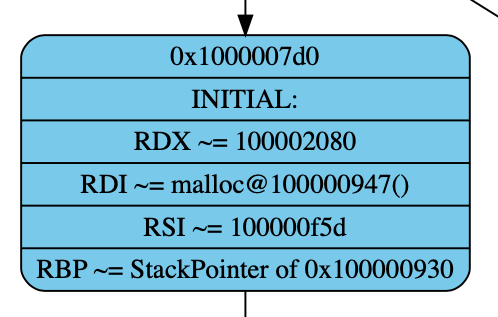
\includegraphics[width=0.27\textwidth]{callgraph2.png}
    }
    \subfloat[Function Constraints]{
       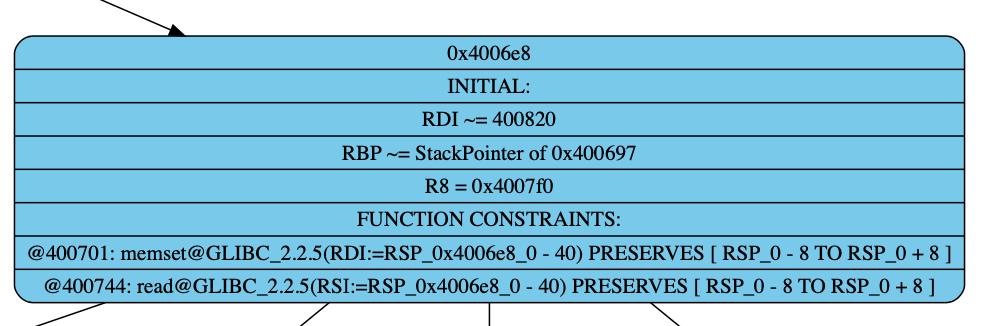
\includegraphics[width=0.73\textwidth]{callgraph1.png}
    }
\caption{Examples of vertices in annotated call graph.}
\label{fig:callgraph1}
\end{figure}


\begin{description}[style=unboxed,leftmargin=0cm,noitemsep,nosep]
\item[INITIAL.] Each function is verified with a certain initialization.
An initialization is an initial predicate such that for any path in the binary, for any state in which the given function is called, the initial predicate holds.
The initialization typically assigns pointer-relevant information to stateparts.
\end{description}
\begin{example}[INITIAL]
Figure~\ref{fig:callgraph1} contains a snippet of the annotated call graph produced using the running example.
This initialization shows that at all times, when function with entry \texttt{1000007d0} is called, register \texttt{RDX} contains a pointer that roughly points to the global data section that contains address \texttt{100002080}. Register \texttt{RDI} contains a pointer produced by \texttt{malloc}. Register \texttt{RBP} contains a pointer to the stack frame of function entry \texttt{100000930}. The initialization does not provide exact information here, but sufficient to know that, e.g., the pointers in registers \texttt{RDX} and \texttt{RDI} point to separate regions.
\end{example}

\begin{description}[style=unboxed,leftmargin=0cm,noitemsep,nosep]
\item[FUNCTION CONSTRAINTS.] 
When a function is called, it may be necessary ot make assumptions over it that cannot be proven.
For external functions, we must make basic assumptions such as calling convention adherence.
But even an internal function may require additional assumptions: it may write above its own stack frame, and in such case assumptions must be made that the return address of the caller is not overwritten.
All these assumptions are summarized as function constraints.
\end{description}
\begin{example}[FUNCTION CONSTRAINTS]
Figure~\ref{fig:callgraph1} contains a snippet of the annotated call graph produced using the example \texttt{rop\_emporium\_ret2win/ret2win}.
Two external functions are called (\texttt{memset} and \texttt{read}).
Both functions are asumed to preserve the top of the stackframe of the caller (\texttt{4006e8}).
In this example, function \texttt{read} may actually \emph{violate} the assumption: it has been provided a pointer to the stackframe of the caller in register \texttt{RSI}, and needs to write more than 32 bytes to violate the assumption.
\end{example}


\begin{description}[style=unboxed,leftmargin=0cm,noitemsep,nosep]
\item[PRECONDITIONS AND ASSERTIONS.] 
Preconditions and assertions for-mulate assumptions over separation of memory writes.
A \emph{precondition} states that two regions in memory are separate whose addresses can be defined in terms of the initial state of the function.
An \emph{assertion} states that two regions are separate at runtime, i.e., specifically during execution of a certain instruction.
\end{description}
\begin{example}[PRECONDITIONS AND ASSERTIONS]
The following precondition:
\begin{center}
StackPointer of \texttt{10000298c} SEP [\texttt{10000388c}, 8]\_0
\end{center}
states that regions based on the stackpointer of the function with entry \texttt{10000298c} are separate from regions based on the pointer \emph{initially} stored in the global variable with address \texttt{10000388c}.
\\
The following assertion:
\begin{center}
@\texttt{100000925}: (\texttt{RDX}\_0 + $\bot$) SEP $\bot_{\mathtt{100000f5d}}$
\end{center}
states that when the instruction at address \texttt{100000925} is executed, the adress of a memory write resolves to the initial value of register \texttt{RDX} plus some unknown value.
The region pointed to by that resolved address is assumed to be separate from regions based in the global data section of address \texttt{100000f5d}.
\end{example}






\fontfamily{cmss}\fontseries{m}\selectfont

\small




%************************************
\vspace{\fill} % ALIGNER EN BAS DE PAGE
%************************************

% Modifier en fonction de l'école
%\noindent
%\color{BleuFonce} \footnotesize 
%Polytech Paris-Saclay \\
%Maison de l'Ingénieur\\
%Bâtiment 620 Université Paris-Saclay\\
%91190 Gif-sur-Yvette, France


\end{document}
